\documentclass[11pt, oneside]{article}   	% use "amsart" instead of "article" for AMSLaTeX format
\usepackage{geometry}                		% See geometry.pdf to learn the layout options. There are lots.
\geometry{letterpaper}                   		% ... or a4paper or a5paper or ... 
%\geometry{landscape}                		% Activate for for rotated page geometry
%\usepackage[parfill]{parskip}    		% Activate to begin paragraphs with an empty line rather than an indent
\usepackage{graphicx}				% Use pdf, png, jpg, or eps� with pdflatex; use eps in DVI mode
								% TeX will automatically convert eps --> pdf in pdflatex		
\usepackage{amssymb}
\usepackage{amsmath}
\usepackage{parskip}
\usepackage{color}

\title{Ellipse:  area}
%\author{The Author}
%\section{}
% \subsection*{R code}
\date{}							% Activate to display a given date or no date

\graphicspath{{/Users/telliott_admin/Dropbox/Tex/png/}}

% \begin{center} 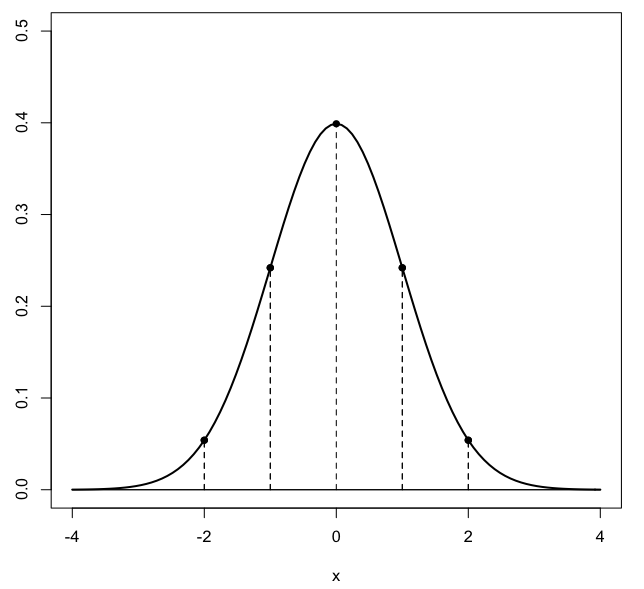
\includegraphics [scale=0.4] {gauss3.png} \end{center}

\begin{document}
\maketitle
\Large
\noindent

The area of an ellipse can be computed in several different ways, all interesting.  The simplest way is rescaling.  In $xy$-coordinates, the formula is
\[ \frac{x^2}{a^2} + \frac{y^2}{b^2} = 1 \]
\[ (\frac{bx}{a})^2 + y^2 = b^2 \]
What this says is that if the $x$ value of each point on the ellipse is re-scaled by a factor of $b/a$, the result is
\[ u = \frac{b}{a}x \]
\[ u^2 + y^2 = b^2 \]
a circle of radius $b$ and area $A = \pi b^2$.  Because the scaling factor is only in the $x$-direction
\[ x = \frac{a}{b}u \]
the area of the original ellipse is bigger by a factor of $a/b$
\[ A = \pi b^2 \ \frac{a}{b} = \pi ab \]
We might also argue as follows.  The area of the ellipse clearly depends on both $a$ and $b$, so we write
\[ A = k a b \]
where $k$ is an unknown constant.  Now, if $a=b$, we obtain
\[ A = k a^2 \]
but this is just a circle, with known area
\[ A = \pi a^2 = k a^2 \]
Hence $k = \pi$ and $A = \pi ab$.

\subsection*{single variable calculus}
Solve the equation of the ellipse for $y$
\[ y = b \sqrt{1 - \frac{x^2}{a^2} } \ dx  \]
We take the positive square root, and integrate from $x = 0 \rightarrow a$, and should obtain $1/4$ the area of the ellipse.
\[ A = 4 b \int \sqrt{1 - \frac{x^2}{a^2} }  \]
The first thing to do is to get rid of the $a$ by substitution.  Let $u = x/a$, so $au = x$ and $a \ du = dx$, then
\[ A = 4 ab \int \sqrt{1 - u^2} \ du  \]
The next step is to recognize that $f(x) = \sqrt{1-u^2}$ is the equation of a circle.  Since we are integrating over the first quadrant, the value of the area is just $\pi/4$.  The whole thing is $\pi$ and we pick up the factor $ab$ from outside to give $A = \pi ab$.

If you failed to see this, you can do a trig substitution.  If $u$ is the side opposite angle $\theta$, and $1$ is the hypotenuse, then 
\[ \sqrt{1-u^2} = \cos \theta \]
\[ u = \sin \theta \]
\[ du = \cos \theta \ \ d\theta \]
and the integral becomes
\[ 4 ab \int \cos^2 \theta \ d\theta  \]
Before we do the integration, consider the changing bounds.  We originally had $x = 0 \rightarrow a$, in changing to $u$ by remembering that
\[ au = x \]
we obtain $u = 0 \rightarrow 1$.  Then, in changing to $\theta$ we have
\[ u = \sin \theta \]
\[ \theta = \sin^{-1} u \]
and we have $\theta = 0 \rightarrow 2\pi$.
I'm not going to do the integral here, but just give the result
\[ \int \cos^2 \theta \ d \theta = \frac{1}{2} (\theta + \sin \theta \cos \theta) \]
(and there are other ways to write it).  But we will take a moment to check that by differentiating
\[ \frac{d}{d \theta} \ \frac{1}{2} (\theta + \sin \theta \cos \theta) \]
\[ =  \frac{1}{2}(1 + \cos^2 \theta - \sin^2 \theta) \]
\[ =  \frac{1}{2}(1 + \cos^2 \theta + \cos^2 \theta - 1) = \cos^2 \theta \]

So we need to evaluate
\[ 4ab \ [ \ \frac{1}{2} (\theta + \sin \theta \cos \theta) \ ] \ \bigg |_0^{\pi/2} \]
Only one term is non-zero and that is $\theta = \pi/2$ at the upper limit.  We obtain
\[ A = 4ab \ (\frac{1}{2}\ \frac{\pi}{2}) = \pi ab \]

\subsection*{Green's Theorem}
State the theorem:
\[ \oint_C \mathbf{F} \cdot \mathbf{r} = \iint_R \nabla \times \mathbf{F} \ dA \]
\[ \int_C M \ dx + N \ dy = \iint_R (N_x - M_y) \ dx \ dy \]
The theorem equates the line integral around a closed path with an area over a region.

To start with, if $\mathbf{F}$ is the gradient of some function, we call such a function the potential, and the integral of the work over a closed path is just zero.

Of course, my favorite example is the area of the ellipse.  

Suppose $N_x - M_y = 1$.  Then the curl integral is the area of the region.  An example would be if $\mathbf{F} = \ \langle M,N \rangle \ = \ \langle -y/2,x/2 \rangle$.  Parametrize the ellipse.
\[ x = a \cos \theta \]
\[ y = b \sin \theta \]
So, for the left hand side we have
\[ \int_C M \ dx + N \ dy = \int_C -\frac{1}{2}y \ dx + \frac{1}{2}x \ dy \]
\[ = \int_0^{2\pi} (-\frac{1}{2})(b \sin \theta) \ (-a \sin \theta) \ d \theta \ + (\frac{1}{2})(a \cos \theta) \ (b \cos \theta) \ d\theta \]
\[ = \int_0^{2\pi} (\frac{ab}{2}\sin^2 \theta + \frac{ab}{2}\cos^2 \theta) \ d \theta = \frac{ab}{2} \int_0^{2\pi} \ d \theta = \pi a b\]

\end{document}  